\documentclass[11pt]{article}

\newcommand{\cnum}{CM146}
\newcommand{\ced}{Winter 2018}
\newcommand{\ctitle}[3]{\title{\vspace{-0.5in}\cnum, \ced\\Problem Set #1: #2}}

\newcommand{\solution}[1]{{{\color{blue}{\bf Solution:} {#1}}}}
\usepackage[usenames,dvipsnames,svgnames,table,hyperref]{xcolor}
\usepackage{amsmath, listings, graphicx}
\renewcommand*{\theenumi}{\alph{enumi}}
\renewcommand*\labelenumi{(\theenumi)}
\renewcommand*{\theenumii}{\roman{enumii}}
\renewcommand*\labelenumii{\theenumii.}
\graphicspath{{images/}}

\begin{document}
\ctitle{0}{Atibhav Mittal (804598987)}
\title{}
\author{}
\date{}
\maketitle
\vspace{-0.75in}

\section{Problem 1}
\begin{enumerate}
\item Problem 1 \newline

\solution{}
\[
	\frac{\partial y}{\partial x} = (\sin{z}) (e^{-x} - xe^{-x})
\]
\vspace{10cm}
\end{enumerate}

\newpage
\section{Problem 2}

\begin{enumerate}
\item Problem 2a \newline
\solution{}
$$
\begin{pmatrix}
1 & 3
\end{pmatrix}
\begin{pmatrix}
2 \\
3
\end{pmatrix}
= 
\begin{pmatrix}
11
\end{pmatrix}
$$

\item Problem 2b \newline
\solution{}
$$
\begin{pmatrix}
2 & 4 \\
1 & 3
\end{pmatrix}
\begin{pmatrix}
1 \\
3
\end{pmatrix}
=
\begin{pmatrix}
14 \\
10
\end{pmatrix}
$$

\item Problem 2c \newline
\solution{}

Yes, the matrix X is invertible since it has a non-zero determinant \break
$$
\begin{vmatrix}
2 & 4 \\
1 & 3
\end{vmatrix}
= 6 - 4 = 2 
$$
$$
X^{-1} = \frac{1}{2}
\begin{pmatrix}
3 & -4 \\
-1 & 2
\end{pmatrix}
$$

\item Problem 2d \newline
\solution{}
The rank of X is 2 (since it is invertible)
\end{enumerate}

\newpage

\section{Problem 3}
\begin{enumerate}

\item Problem 3a \newline
\solution{}
$$
Sample\quad Mean = \frac{1 + 1 + 0 + 1 + 0}{5} = \frac{3}{5} = 0.6
$$


\item Problem 3b \newline
\solution{}
$$
Sample\quad Variance = \frac{1.3}{5} = 0.26
$$

\item Problem 3c \newline
\solution{}
Probability of observing this pattern is:
$$
\frac{1}{2^5} = \frac{1}{32}
$$

\item Problem 3d \newline
\solution{}
Let the probability 
$$
P(X_{i} = 0) = p
$$
$$
P(X_{i} = 1) = (1 - p)
$$
Probability of pattern (since all events are independent):
$$
X = \frac{1}{1-p} \cdot \frac{1}{1-p} \cdot \frac{1}{p} \cdot \frac{1}{1-p} \cdot \frac{1}{p} = \frac{1}{p^2 - 3p^3 + 3p^4 - p^5}
$$
Taking the derivative of the above equation, and setting it to zero gives us the following equation
$$
- {(p-1)}^2 (5p - 2) = 0
$$
$$
\Rightarrow p = \frac{2}{5}
$$
$$
\Rightarrow P(X_{i} = 1) = \frac{3}{5}
$$

\item Problem 3e \newline
\solution{}
$$
P(X = T | Y = b) = \frac{0.1}{0.1 + 0.15} = \frac{0.1}{0.25} = \frac{2}{5}
$$
\end{enumerate}

\newpage
\section{Problem 4}
\begin{enumerate}

\item 
\solution{}
False

\item 
\solution{}
True

\item 
\solution{}
False

\item 
\solution{}
False

\item
\solution{}
True

\end{enumerate}

\newpage

\section{Problem 5}

(a) - (v) \newline
(b) - (iv) \newline
(c) - (ii) \newline
(d) - (i) \newline
(e) - (iii) 

\newpage
\section{Problem 6}
\begin{enumerate}
\item Problem 6a \newline
\solution{}
Mean of a Bernoulli random variable = p \newline
Variance of a Bernoulli random variable = p(1 - p)

\item Problem 6b \newline
\solution{}
$$var(X) = \sigma ^ 2$$
$$var(2X) = 4 \sigma ^ 2$$
$$var(X + 2) =  \sigma ^ 2$$
\end{enumerate}

\newpage
\section{Problem 7}
\begin{enumerate}
\item
\begin{enumerate}
\item 
\solution{}
Both f(n) = O(g(n)) and g(n) = O(f(n)) are true

\item
\solution{}
f(n) = O(g(n))

\item 
\solution{}
f(n) = O(g(n))
\end{enumerate}


\item Problem 7b \newline
\solution{}
\begin{lstlisting}
findTransition(Array a, startIndex, endIndex):
	middle = (startIndex + endIndex ) / 2
	if(a[middle] is 0 and a[middle + 1] is a 1):
		// transition point found
		return middle
	else if (a[middle] and a[middle] are both 0):
		// both elements in the center are 0, so search in 
			// the right half of the array
		return findTransition(a, middle, endIndex)
		
	else: // both elements at a[middle] and a[middle + 1] 
			// are 1, so search in left half of the array
		return findTransition(a, 0, middle)
\end{lstlisting}
\begin{verbatim}		
Correctness:
	Suppose the transition from 0s to 1s happens at index i (i > n/2), where n 
	is the number of elements in the array. Since the transition happens in the 
	second half of the array, all elements to the left of the middle index are 0s, 
	and we only need to search the right half of the array. On the recursive call, 
	the problem remains the same but is a smaller problem. Similarly, it can be 
	shown that the algorithm will always examine the correct index if i < n/2. If 
	the transition happens in the dead center, then this will be found on the first
	call and the result returned. Hence, the algorithm is correct.

Runtime:
	At every recursive call, the problem size is reduced by half. This can 
	be given by the recurrence relation:
		T(n) = T(n/2) + O(1)
	The solution to this recurrence relation is an algorithm of O(log n) time. 
\end{verbatim}



\end{enumerate}

\newpage
\section{Problem 8}
\begin{enumerate}
\item Problem 8a \newline
\solution{}
$$
	E[XY] = \sum_{x,y} xy p_{X,Y}(x,y)
$$
Since X, Y are independent: 
$$
	E[XY] = \sum_{x,y} xy p_{X}(x) p_{Y}(y) \qquad $$
$$
	E[XY] = \sum_{x} x p_{X}(x) \sum_{y} y p_{Y}(y)
$$
$$
	E[XY] = E[X]E[Y]
$$

\item Problem 8b (i) \newline
\solution{}
Number of times 3 shows up on a fair die rolled 6000 times is = Binomial (6000, $\frac{1}{6}$) \newline
Expectation = $ np = 6000 \cdot \frac{1}{6} = 1000 $

\item Problem 8b (ii) \newline
\solution{}
Using the central limit theorem, as n$\rightarrow \infty$,
distribution approaches N(0, $\sigma^2$). \newline
For a fair coin, $\sigma^2 = p(1 - p) = \frac{1}{2} ^2 = \frac{1}{4}$ \newline
Hence, the distribution becomes N(0, $\frac{1}{4}$)
\end{enumerate}

\newpage
\section{Problem 9}
\subsection{9a}
\begin{enumerate}
\item Problem 9a (i) 
\solution{}
\newline
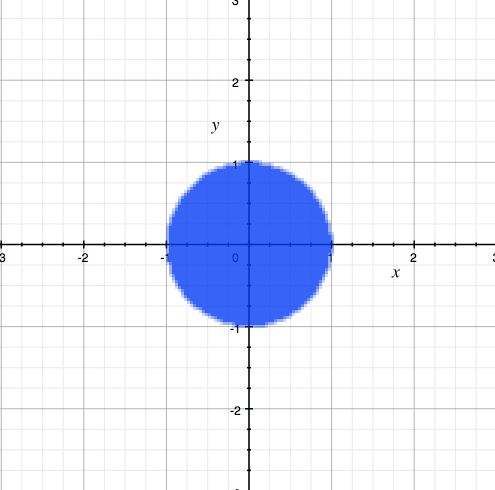
\includegraphics[scale=0.4]{9a(i)}

\item Problem 9a (ii)
\solution{}
\newline
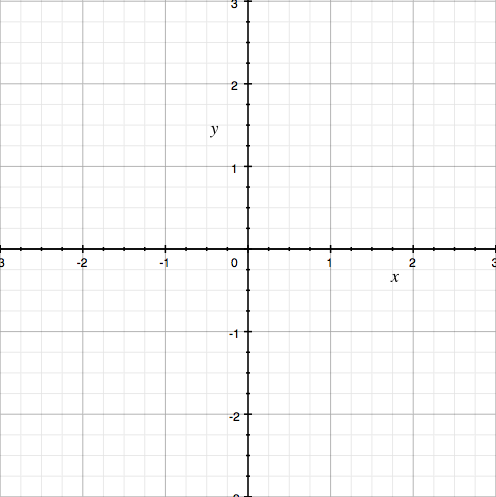
\includegraphics[scale=0.4]{9a(ii)}

\item Problem 9a (iii) 
\solution{}
\newline
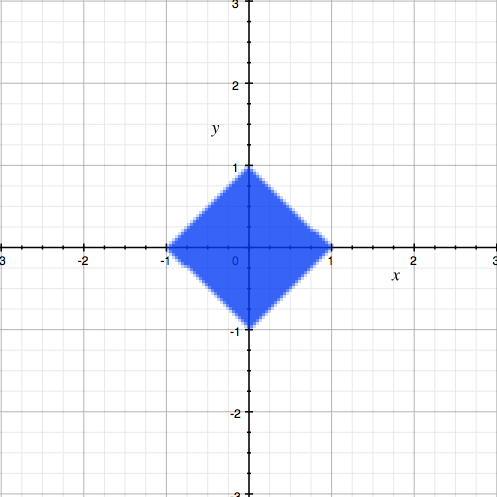
\includegraphics[scale=0.4]{9a(iii)}

\item Problem 9a (iv)
\solution{}
\newline
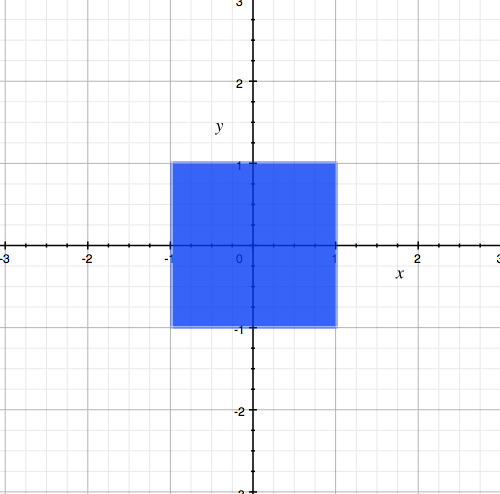
\includegraphics[scale=0.4]{9a(iv)}

\end{enumerate}

\subsection{9b}
\begin{enumerate}
\setcounter{enumi}{1}

\item
\begin{enumerate}
\item 9b (i) \newline
\solution{}
The eigenvector $\vec{v}$ of a square matrix, $A$ is a vector such that $$ A\vec{v} = \lambda \vec{v}$$
The scalar $\lambda$ is called an eigenvalue of the square matrix.

\item 9b (ii) \newline
\solution{}
The eigenvalues can be found by setting the determinant of the matrix $ A - \lambda I$ equal to 0
$$
\begin{vmatrix}
2 - \lambda & 1 \\
1 & 2 - \lambda
\end{vmatrix}
 = 0
$$
$$
(2 - \lambda)^2 - 1 = 0
$$
$$
\lambda ^ 2 - 4 \lambda + 3 = 0
$$
$$
(\lambda - 3)(\lambda - 1) = 0
$$
$$
\Rightarrow \lambda = 3, 1
$$
To find the eigenvectors, we find a vector such that $(A - \lambda I)\vec{v} = 0 $
\newline
For $\lambda = 3$
$$
\begin{pmatrix}
-1 & 1 \\
1 & -1 
\end{pmatrix}
\vec{x} = 0
$$
$$
\vec{x} = 
\begin{bmatrix}
1 \\
1
\end{bmatrix}
$$
\newline
For $\lambda = 1$
$$
\begin{pmatrix}
1 & 1 \\
1 & 1
\end{pmatrix}
\vec{x} = 0
$$
$$
\vec{x} = 
\begin{bmatrix}
1 \\
-1
\end{bmatrix}
$$

\item Problem 9b (iii) \newline
\solution{}
Consider a matrix A, with eigenvectors $v_{1}, v_{2}, ... , v_{n}$ and eigenvalues 
$\lambda_{1}, \lambda_{2}, ..., \lambda_{n}$. \newline
To prove the required statement we use induction. \newline
Base case:
The base case is trivial. For the matrix A, we have the eigenvectors 
$v_{1}, v_{2}, ... , v_{n}$ and eigenvalues $\lambda_{1}, \lambda_{2}, ..., \lambda_{n}$ \newline
Induction Step: \newline
Assume that for $A^k$, the eigenvectors are $v_{1}, v_{2}, ... , v_{n}$ and eigenvalues $\lambda_{1}^k, \lambda_{2}^k, ..., \lambda_{n}^k$ \newline
We need to show this for $A^{k+1}$ \newline
Consider any eigenvector $v_{i}$ of $A^{k}$, with eigenvalue $\lambda_{i}^{k}$
$$ A^k v_{i} = \lambda_{i}^{k} v_{i}$$ 
$$ A^{k+1} v_{i} = A A^{k} v_{i} = A \lambda_{i}^{k} v_{i} = \lambda_{i}^{k} A v_{i} = \lambda_{i}^{k+1} v_{i}$$
$\Rightarrow A^{k+1}$ has eigenvalue $\lambda_{i}^{k+1}$ and eigenvector $v_{i}$. \newline
Hence, proved by the principle of mathematical induction.
\end{enumerate}

\item Problem 9c \newline
\begin{enumerate}
\item 9c (i) \newline
\solution{} 
$$
\frac{\partial (a^T x)}{\partial x} = a^T
$$

\item 9c (ii) \newline
\solution{}
$$
\frac{\partial (x^T Ax)}{\partial x} = x^T (A^T + A)
$$

\end{enumerate}

\item Problem 9d \newline
\begin{enumerate}
\item 9d(i) \newline
\solution{}
Consider two points $x_{1}, x_{2}$ that lie on the line.
$$ w^T x_{1} + b = 0$$
$$ w^T x_{2} + b = 0$$
Subtracting second equation from first equation,
$$ w^T x_{1} - w^T x_{2} = 0$$
$$ w^T (x_{1} - x_{2}) = 0 $$
$$ \vec{w} \cdot (\vec{x_{1}} - \vec{x_{2}}) = 0$$
Hence, w is orthogonal to the line passing through $x_{1}$ and $x_{2}$.

\item 9d(ii) \newline
\solution{}
Let w = ($a_{1}, a_{2}, ... a_{n}$) and x = ($x_{1}, x_{2}, ..., x_{n}$)
$$ w^T x + b = a_{1} x_{1} + a_{2} x_{2} + .... + a_{n} x_{n} + b $$
$$ ||w||_{2} = \sqrt{a_{1}^2 + a_{2}^2 + ... + a_{n}^2}$$
Distance from (0,0,0...,0) = $\frac{0 + 0 + ... + b}{\sqrt{a_{1}^2 + a_{2}^2 + ... + a_{n}^2}} = \frac{b}{||w||_2}$
\end{enumerate}
\end{enumerate}

\newpage
\section{Problem 10}
\begin{enumerate}
\item
\solution{} \newline
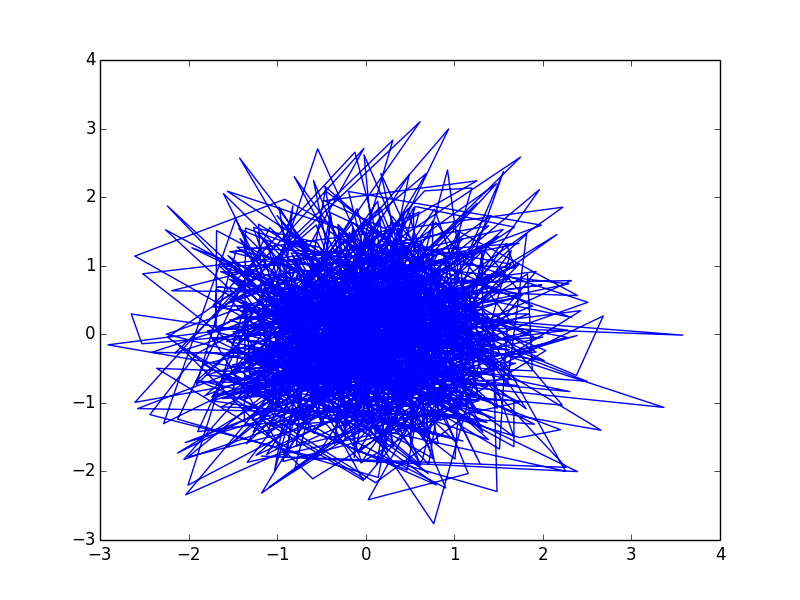
\includegraphics[scale=0.5]{10a.png}

\item 
\solution{} \newline
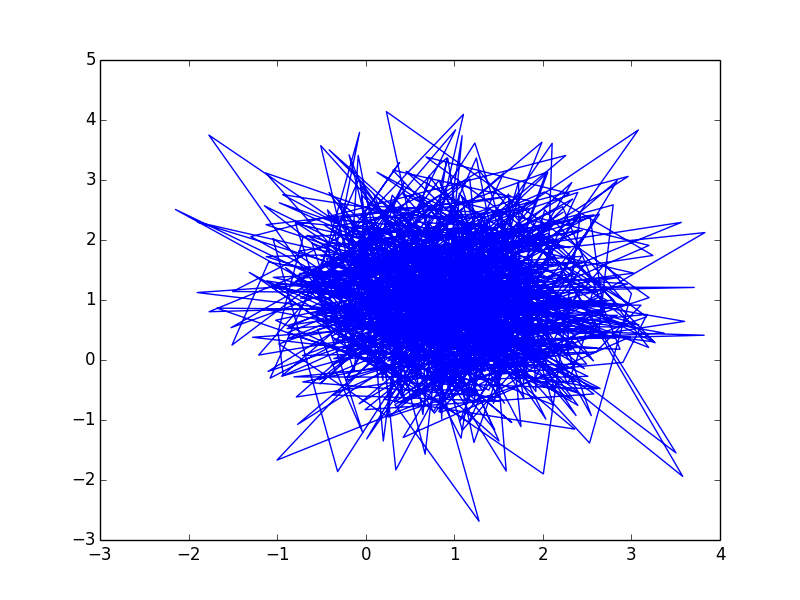
\includegraphics[scale=0.5]{10b.png}

\item 
\solution{} \newline
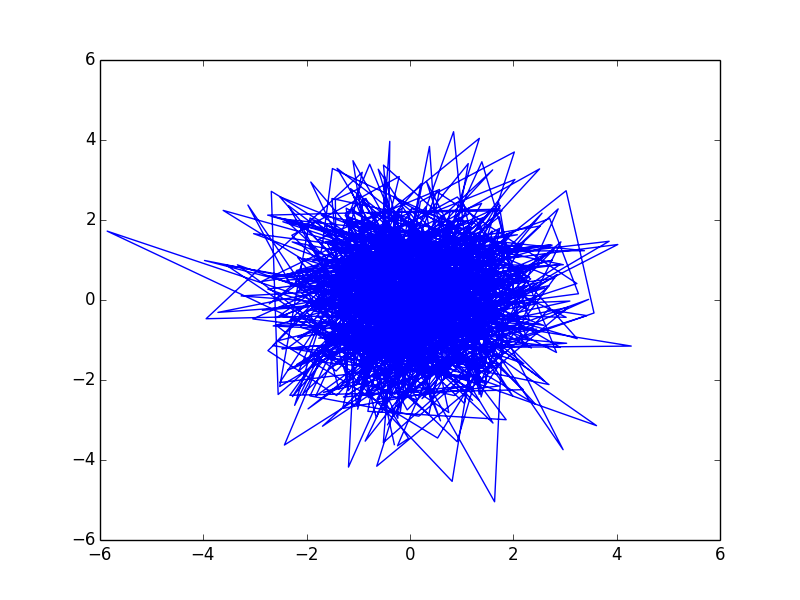
\includegraphics[scale=0.5]{10c.png}

\item
\solution{} \newline
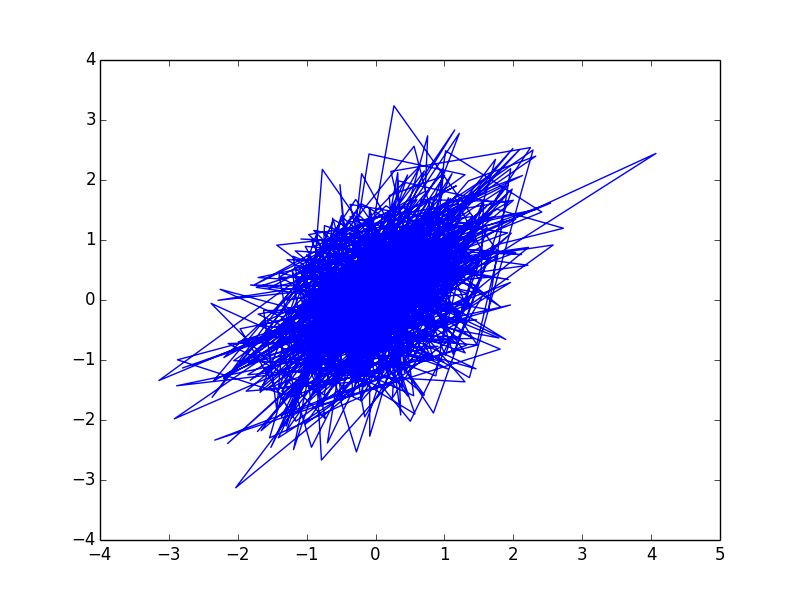
\includegraphics[scale=0.5]{10d.png}

\item
\solution{} \newline
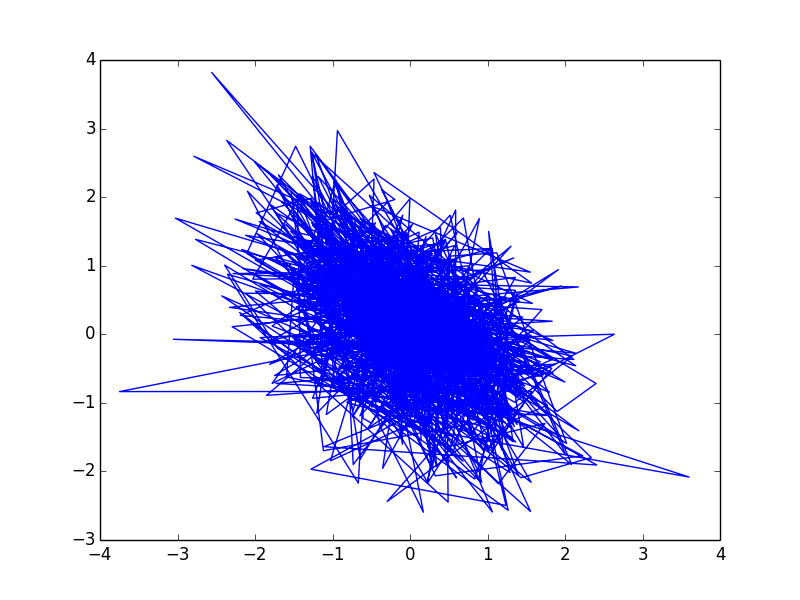
\includegraphics[scale=0.5]{10e.png}
\end{enumerate}

\newpage
\section{Problem 11}
\solution{}
\begin{lstlisting}[language=Python]
import numpy as np 

A = np.array([[1, 0], [1, 3]])

eigenvalues, eigenvectors = np.linalg.eig(A)%

max_eigenval_index = np.argmax(eigenvalues)

max_eigenvector = eigenvectors[max_eigenval_index]

print(max_eigenvector)
\end{lstlisting}

\newpage
\section{Problem 12}
\begin{enumerate}
\item Yelp Open Dataset
\item https://www.yelp.com/dataset
\item The dataset contains details of a business (such as address, number of reviews etc. ) and reviews of the business. It also contains the number of checkins on the business every hour. This can be used to predict the number of checkins in the future for each business. 
\item 4.7 million reviews, so the dataset contains 4.7 million rows
\item Features: Number of check-ins for the business, number of useful votes, number of funny votes, number of cool votes, star rating, number of complaints
\end{enumerate}

\end{document}
